\chapter{Fully Automatic Stream Management For Multi-Streamed SSDs Using Program Contexts} 
\label{chap:PCstream}

\section{Overview}

In flash-based SSDs, garbage collection (GC) is inevitable because NAND flash
memory does not support in-place updates.  Since the efficiency of garbage
collection significantly affects  both the performance and lifetime of SSDs,
garbage collection has been extensively investigated so that the garbage
collection overhead can be reduced ~\cite{DAC, WriteAmplification, GCGreedy,
GCVictim, GCTTFlash, HotCold}.  For example, hot-cold separation techniques are
commonly used inside an SSD so that quickly invalidated pages are not mixed
with long-lived data in the same block.   For more efficient garbage
collection, many techniques also exploit host-level I/O access characteristics
which can be used as useful hints on the efficient data separation inside the
SSD~\cite{JiTGC, ShadowGC}.

Multi-streamed SSDs provide a special interface mechanism for a host system,
called streams\footnote{In this dissertation, we use ``streams'' and ``external
streams'' interchangeably.}, which data separation decisions {\it on the
host level} can be delivered to SSDs~\cite{T10, MultiStream}.  When the host
system assigns two data $D_1$ and $D_2$ to different streams $S_1$ and $S_2$,
respectively, a multi-streamed SSD places $D_1$ and $D_2$ in different blocks,
which belong to $S_1$ and $S_2$, respectively.  When $D_1$ and $D_2$ have
distinct update patterns, say, $D_1$ with a short lifetime and $D_2$ with a
long lifetime, allocating $D_1$ and $D_2$ to different streams can be helpful
in minimizing the copy cost of garbage collection by separating hot data from
cold data.  Since data separation decisions can be made more intelligently on
the host level over on the SSD level, when streams are properly managed, they
can significantly improve both the performance and lifetime of flash-based
SSDs~\cite{MultiStream, Level,vStream, FStream, AutoStream}.  We assume that a
multi-streamed SSD supports $m$+1 streams, $S_0$, ..., $S_{m}$.

In order to maximize the potential benefit of multi-streamed SSDs in practice,
several requirements need to be satisfied both for stream management and for
SSD stream implementation.  First, stream management should be supported in a
fully automatic fashion over general I/O workloads without any manual work.
For example, if an application developer should manage stream allocations {\it
manually} for a given SSD, multi-streamed SSDs are difficult to be widely
employed in practice.   Second, stream management techniques should have no
dependency on the number of available streams.  If stream allocation decisions
have some dependence on the number of available streams,  stream allocation
should be modified whenever the number of streams in an SSD changes.  Third,
the number of streams supported in an SSD should be sufficient to work well
with multiple concurrent I/O workloads.  For example, with 4 streams, it would
be difficult to support a large number of I/O-intensive concurrent tasks.  

Unfortunately, to the best of our knowledge, no existing solutions  for
multi-streamed SSDs meet all these requirements.  Most existing
techniques~\cite{MultiStream, Level, vStream, FStream} require programmers to
assign streams at the application level with manual code modifications.
\textsf{\small AutoStream}~\cite{AutoStream} is the only known automatic
technique that supports stream management in the kernel level without manual
stream allocation.  However, since \textsf{\small AutoStream} predicts data
lifetimes using the update frequency of the logical block address (LBA), it
does not work well with append-only workloads (such as
RocksDB~\cite{RocksDB} or Cassandra~\cite{Cassandra})
and write-once workloads (such as a Linux kernel build).  Unlike conventional
in-place update workloads where data written to the same LBAs often show strong update
locality, append-only or write-once workloads make it impossible to predict data lifetimes
from LBA characteristics such as the access frequency.

In this dissertation, we propose a {\it fully-automatic} stream management technique,
called \textsf{\small PCStream}, which works efficiently over general I/O
workloads including append-only, write-once as well as in-place update workloads.   
The key insight behind
\textsf{\small PCStream} is that stream allocation decisions should be made at
a higher abstraction level where {\it I/O activities}, not LBAs, can be
meaningfully distinguished.  For example, in RocksDB, if we can tell whether
the current I/O is a part of a logging activity or a compaction activity, stream
allocation decisions can be made a lot more efficiently over when only LBAs of
the current I/O is available.   

In \textsf{\small PCStream}, we employ a write program context\footnote{
Since we are interested in write-related system calls such as {\tt write()} in
Linux, we use {\it write program contexts} and {\it program contexts}
interchangeable where no confusion arises.} as such a higher-level
classification unit for representing I/O activity regardless of the type of I/O
workloads.  A program context (PC)~\cite{PC, PC2}, which uniquely represents an
execution path of a program up to a write system call, is known to be effective
in representing dominant I/O activities~\cite{PCHa}.  Furthermore, most
dominant I/O activities tend to show distinct data lifetime characteristics.
By identifying dominant I/O activities using program contexts during run time,
\textsf{\small PCStream} can automate the whole process of stream allocation
within the kernel with no manual work.  In order to seamlessly support various
SSDs with different numbers of streams, \textsf{\small PCStream} groups program
contexts with similar data lifetimes depending on the number of supported
streams using the k-means clustering algorithm~\cite{kmeans}.  Since program
contexts focus on the semantic aspect of I/O execution as a lifetime
classifier, not on the low-level details such as LBAs and access patterns,
\textsf{\small PCStream} easily supports different I/O workloads regardless of
whether it is update-only or append-only.   

Although many program contexts show that their data lifetimes are narrowly
distributed, we observed that this is not necessarily true because of several
reasons.  For example, when a single program context handles multiple types of
data with different lifetimes, data lifetime distributions of such program
contexts  have rather large variances.  In \textsf{\small PCStream}, when such
a program context {\it $PC_j$} is observed (which was mapped to a stream {\it
$S_k$}), the long-lived data of {\it $PC_j$} are moved to a different stream
{\it $S_{k'}$} during GC.  The stream {\it $S_{k'}$} prevents the long-lived
data of the stream {\it $S_k$} from being mixed with future short-lived data of
the stream {\it $S_k$}.

When several program contexts have a large variance in their data lifetimes,
the required number of total streams can quickly increase to distinguish data
with different lifetimes.
%if streams can efficiently distinguish data with different lifetimes.
In order to effectively increase the number of streams, we propose a new stream
type, called an internal stream, which can be used only for garbage collection.
Unlike external streams, internal streams can be efficiently implemented at low
cost without increasing the SSD resource budget.  In the current version of
\textsf{\small PCStream}, we create the same number of internal streams as the
external streams, effectively doubling the number of available streams. 

In order to evaluate the effectiveness of \textsf{\small PCStream}, we have
implemented \textsf{\small PCStream} in the Linux kernel (ver. 4.5) and
extended a Samsung PM963 SSD to support internal streams.  Our experimental
results show that \textsf{\small PCStream} can reduce the GC overhead as much
as a manual stream management technique while requiring no code modification.
Over \textsf{\small AutoStream}, \textsf{\small PCStream} improves the average
IOPS by 28\% while reducing the average WAF by 49\%.


\section{Motivation}
\subsection{No Automatic Stream Management for General I/O Workloads}
%\subsection{\note{No Automatic Stream Management}}
Most existing stream management techniques~\cite{MultiStream,Level,vStream} 
require programmers to manually allocate streams for their applications.
For example, 
in both \textsf{\small ManualStream\footnote{For brevity, we denote the manual stream allocation
method used in ~\cite{MultiStream} by \textsf{\scriptsize ManualStream}.}}~\cite{MultiStream} and 
~\cite{Level}, there is no systematic guildeline on how to
allocate streams for a given application. 
The efficiency of stream allocations largely depends on the programmer's 
understanding and expertise on data temperature ({\it i.e.}, frequency of updates)
and internals of database systems.
Furthermore, many
techniques also assume that the number of streams is known {\it a priori}.  
Therefore, when an SSD with a different number of streams is used, 
these techniques need to re-allocate streams manually.
\textsf{\small vStream}~\cite{vStream} 
is an exception to this 
restriction by allocating streams to virtual streams, not external streams.  
However, even in \textsf{\small vStream}, virtual stream allocations are left to
programmer's decisions.

Although \textsf{\small FStream}~\cite{FStream} and \textsf{\small AutoStream}~\cite{AutoStream}
may be considered 
as automatic stream management techniques,
their applicability is quite limited.
\textsf{\small FStream}~\cite{FStream} can be useful for separating file system metadata but it does not
work for the user data separation.
\textsf{\small AutoStream}~\cite{AutoStream} is the only known technique that works in a 
fully automatic fashion by making stream allocation decisions within 
the kernel.
However, since \textsf{\small AutoStream} predicts data lifetimes using the
access frequency of the same LBA, \textsf{\small AutoStream} does not work well 
when no apparent {\it locality} on LBA accesses exists in applications.  
For example, in recent data-intensive applications 
such as RocksDB~\cite{RocksDB} and Cassandra~\cite{Cassandra}, 
majority of data are written in an append-only manner,
thus no LBA-level locality can be detected inside an SSD.

\begin{figure*}[t]
	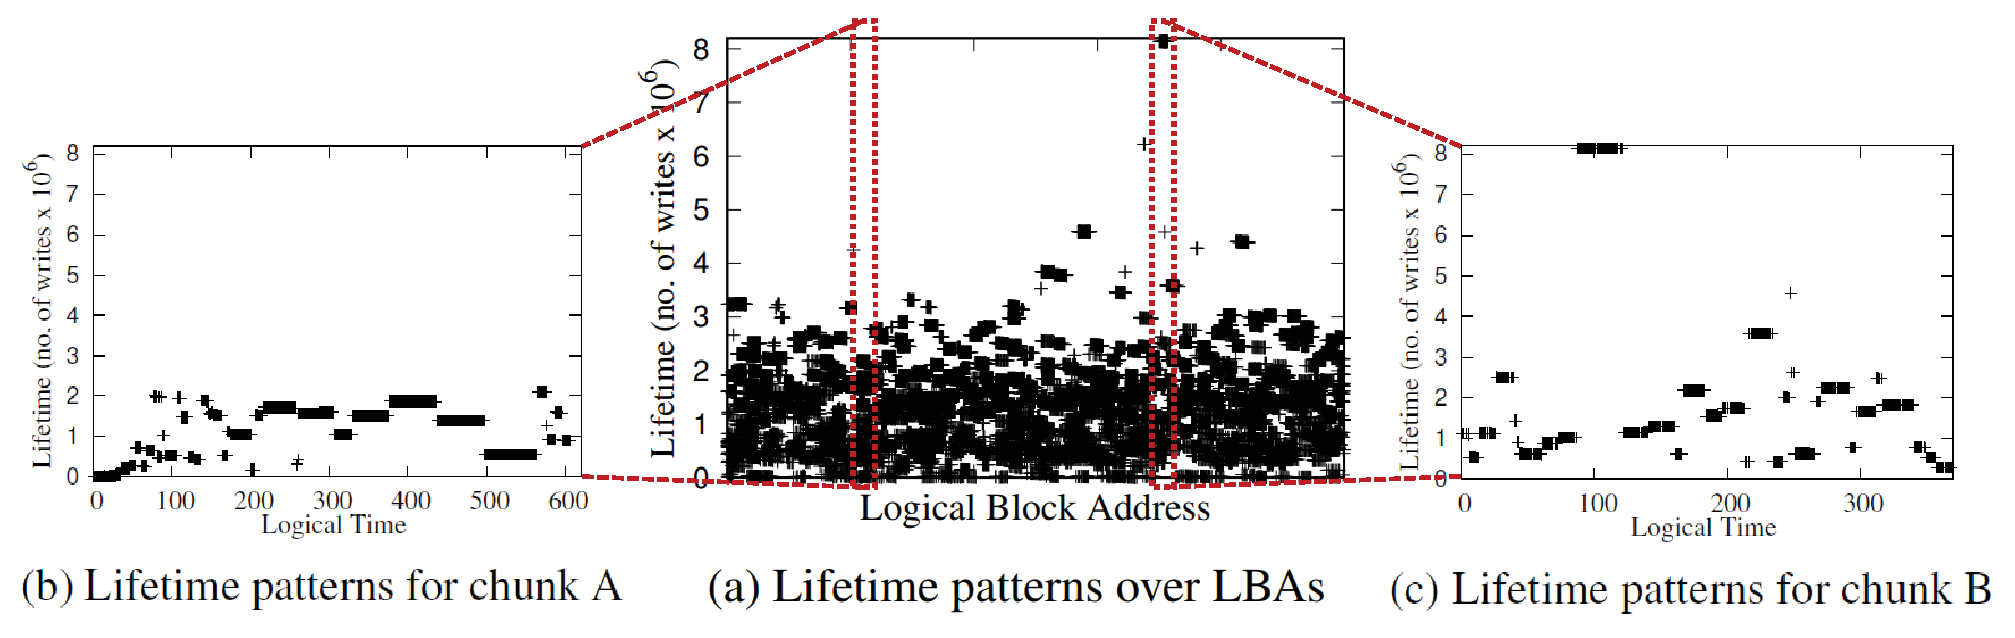
\includegraphics[width=\linewidth]{figure/pcstream/fig1}
	\caption{Lifetime distributions of append-only workload over addresses and times.}
	\label{fig:lba_lifetime}
\end{figure*}


In order to illustrate a mismatch between an LBA-based data separation technique and 
append-only workloads, we analyzed the write pattern of 
RocksDB~\cite{RocksDB}, which is a
popular key-value store based on the LSM-tree algorithm~\cite{LSM}.
Fig.~\ref{fig:lba_lifetime}(a) shows how LBAs may be related 
to data lifetimes in RocksDB.  
We define the lifetime of data as the interval length (in terms of
the logical time based on the number of writes) between
when the data is first written and when the data is invalidated
by an overwrite or a TRIM command~\cite{TRIM}.
As shown in Fig.~\ref{fig:lba_lifetime}(a), 
there is no strong correlation between LBAs and their lifetimes in RocksDB.  

We also analyzed 
if the lifetimes of LBAs change under some predictable patterns over time 
although the overall lifetime distribution shows large variances.
Figs.~\ref{fig:lba_lifetime}(b) and~\ref{fig:lba_lifetime}(c) show
scatter plots of data lifetimes over the logical time 
for two specific 1-MB chunks with 256 pages. 
As shown in Figs.~\ref{fig:lba_lifetime}(b) and~\ref{fig:lba_lifetime}(c), 
for the given chunk, the lifetime of data written to the chunk 
varies in an unpredictable fashion.  
For example, at the logical time 10 in Fig.~\ref{fig:lba_lifetime}(b), 
the lifetime was 1 but it increases about 
2 million around the logical time 450 
followed by a rapid drop around the logical time 500. 
Our workload analysis using RocksDB strongly suggests that under append-only workloads, 
LBAs are not useful in predicting data lifetimes reliably.
In practice, the applicability of LBA-based data separation techniques is quite 
limited to a few cases only when the LBA access
locality is obvious in I/O activities such as updating metadata files or log files.  
In order to support {\it general} I/O workloads in an automatic fashion, stream 
management decisions should be based on higher-level information
which do not depend on lower-level details such as write patterns based on LBAs.

\subsection{Limited Number of Supported Streams}
\label{sec:limitedstreams}

\begin{figure*}[t]
	\centering
	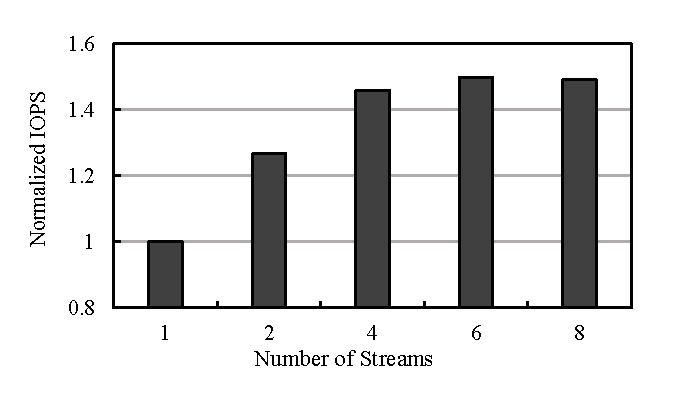
\includegraphics[width=0.8\textwidth]{figure/pcstream/stream_perf}
	\caption{IOPS changes over the number of streams.}
	\label{fig:stream_perf}
\end{figure*}

One of the key performance parameters in multi-streamed SSDs is the number of
available streams in SSDs.  Since the main function of  streams is to separate
data with different lifetimes so that they are not mixed in the same block, it
is clear that the higher the number of streams, the more efficient the
performance of multi-streamed SSDs.  For example, Fig.~\ref{fig:stream_perf}
shows how IOPS in RocksDB changes as the number of streams increases on a
Samsung PM963 multi-streamed SSD with 9 streams.  The \texttt{db\_bench}
benchmark was used for measuring IOPS values with streams manually allocated.
As shown in Fig.~\ref{fig:stream_perf}, the IOPS is continuously improving
until 6 streams are used when dominant I/O activities with different data
lifetimes are sufficiently separated.  In order to support a large number of
streams, both the SBC-4 and NVMe revision 1.3, which define the multi-stream
related specifications, allow up to 65,536 streams~\cite{T10, NVMe}.  However,
the number of streams supported in commercial SSDs is quite limited, say, 4 to
16~\cite{MultiStream, Level, AutoStream}, because of several implementation
constraints on the backup power capacity and fast memory size.

These constraints are directly related to a write buffering mechanism that is
commonly used in modern SSDs.   In order to improve the write throughput while
effectively hiding the size difference between the FTL mapping unit and the
flash program unit, host writes are first buffered before they are written to
flash pages in a highly parallel fashion for high performance.  Buffering host
writes temporarily inside SSDs, however, presents a serious data integrity risk
for storage systems when a sudden power failure occurs.  In order to avoid such
critical failures, in data centers or storage servers where multi-streamed SSDs
are used, SSDs use tantalum or electrolytic capacitors as a backup power
source.  When a main power is suddenly failed, the backup power is used to
write back the buffered data reliably.  Since the capacity of backup power is
limited because of the limited PCB size and its cost, the maximum amount of
buffered data is also limited.  In multi-streamed SSDs where each stream needs
its own buffered area, the amount of buffered data increases as the number of
streams increases.  The practical limit in the capacity of backup power,
therefore, dictates the maximum number of streams as well.

The limited size of fast memory, such as TCM~\cite{TCM} or SRAM, is another
main hurdle in increasing the number of streams in multi-streamed SSDs.  Since
multi-stream related metadata which includes data structures for write
buffering should be accessed quickly as well as frequently, most SSD
controllers implement data structures for supporting streams on fast memory
over more common DRAM.  Since the buffered data is the most recent one for a
given LBA, each read request needs to check if the read request should be
served from the buffered data or not.  In order to support a quick checkup of
buffered data, probabilistic data structures such as a bloom filter can be used
along with other efficient data structures, for accessing LBA addresses of
buffered data and for locating buffer starting addresses.   Since the latency
of a read request depends on how fast these data structures can be accessed,
most SSDs place the buffering-related data structure on fast memory.
Similarly, in order to quickly store buffered data in flash chips, these data
structure should be placed on fast memory as well.  However, most SSD
manufacturers are quite sensitive in increasing the size of fast memory because
it may increase the overall SSD cost.   A limited size of fast memory,
unfortunately, restricts the number of supported streams quite severely.

\section{Automatic I/O Activity Management}
\label{sec:programcontext}
In developing an efficient data lifetime separator for general I/O workloads,
our key insight was that in most applications, the overall I/O behavior of
applications is decided by a few dominant I/O activities ({\it e.g.}, logging and
flushing in RocksDB).  Moreover, data written by dominant I/O activities tend
to have distinct lifetime patterns.  Therefore, if such dominant I/O activities
of applications can be automatically detected and distinguished each other in
an LBA-{\it oblivious} fashion, an automatic stream management technique can be
developed for widely varying I/O workloads including append-only workloads.

In this dissertation, we argue that a program context can be used to build an
efficient general-purpose classifier of dominant I/O activities with different
data lifetimes.  Here, a PC represents an execution path of an application
which invokes write-related system call functions such as {\tt write()} and
{\tt writev()}.  There could be various ways of extracting PCs, but the most
common approach~\cite{PC, PC2} is to represent each PC with its PC signature
which is computed by summing program counter values of all the functions along
the execution path which leads to a write system call.

%we represent the PC by summing program counter values of
%all the functions along the execution path which leads to a write system call.

%\subsection{Program Context as a Unit of Lifetime Classification}
\subsection{PC as a Unit of Lifetime Classification for General I/O Workloads}
In order to illustrate that using PCs is an effective way to distinguish I/O
activities of an application and their data lifetime patterns, we measured data
lifetime distributions of PCs from various applications with different I/O
workloads.  In this section, we report our evaluation results for three
applications with distinct I/O activities: RocksDB~\cite{RocksDB},
SQLite~\cite{SQLite}, and GCC~\cite{GCC}.  RocksDB shows the append-only
workload while SQLite shows a workload that updates in place.  Both database
workloads are expected to have distinct I/O activities for writing log files
and data files.  GCC represents an extensive compiler workload ({\it e.g.},
compiling a Linux kernel) that generates many short-lived temporary files ({\it
e.g.}, \texttt{.s}, \texttt{.d}, and \texttt{.rc} files) as well as some
long-lived files ({\it e.g.}, object files and kernel image files).

%\textcolor{red}{(TODO: 갑자기
%lifetime 이야기가 나옴. 없애도 큰 문제가 없을 듯...) \sout{Note that using a
%program context to distinguish data lifetimes is not new. For example, Ha {\it
%et al.} proposed a data separation technique based on the program
%context~\cite{PCHa}.  However, their work was neither designed for append-only
%workloads nor for modern multi-streamed SSDs.}}

\begin{figure*}[!t]
\centering
	\subfloat[RocksDB: Logging]{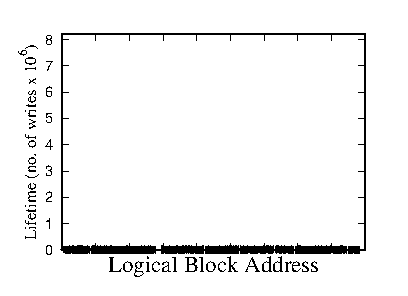
\includegraphics[width=0.3\textwidth]{figure/pcstream/pcID_2_new.eps}} % data from 4/03031953 
	\hspace{2pt}
	\subfloat[RocksDB: Flushing]{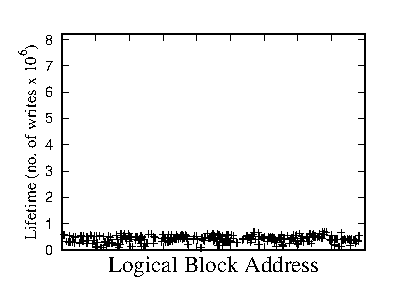
\includegraphics[width=0.3\textwidth]{figure/pcstream/pcID_3_new.eps}}
	\hspace{2pt}
	\subfloat[RocksDB: Compaction]{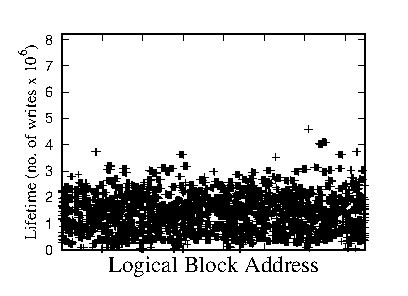
\includegraphics[width=0.3\textwidth]{figure/pcstream/pc_3_new.eps}}  % data from 4/03040047
	\hfill
	\subfloat[SQLite: Logging]{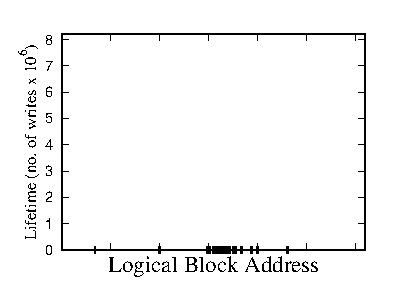
\includegraphics[width=0.3\textwidth]{figure/pcstream/sqlite_pcID_6_new.eps}}
	\hspace{2pt}
	\subfloat[SQLite: Updating]{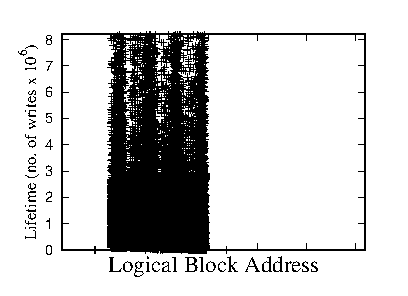
\includegraphics[width=0.3\textwidth]{figure/pcstream/sqlite_pcID_1_new.eps}}
	\hspace{2pt}
	\subfloat[GCC: Outputting Temp]{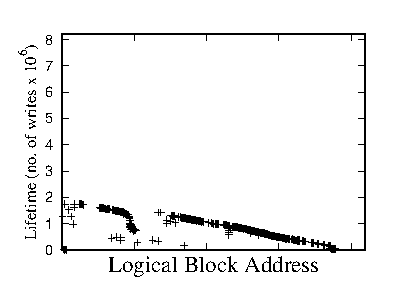
\includegraphics[width=0.3\textwidth]{figure/pcstream/gcc_pcID_1_new.eps}}
	\hfill
	\subfloat[GCC: Outputting Executable]{
\includegraphics[width=0.3\textwidth]{figure/pcstream/gcc_pcID_8_new.eps}}
\caption{Data lifetime distributions of dominant I/O activities in RocksDB, SQLite and GCC.} 
\label{fig:types_and_PCs}
\end{figure*}


To confirm our hypothesis that data lifetimes can be distinguished by tracking
dominant I/O activities and a PC is a useful unit of classification for
different I/O activities, we have analyzed how well PCs work for RocksDB,
SQLite and GCC.  Fig.~\ref{fig:types_and_PCs} shows data lifetime distributions
of dominant I/O activities which were distinguished by computed PC values.  As
expected, Fig.~\ref{fig:types_and_PCs} validates that dominant I/O activities
show distinct data lifetime distributions over the logical address space.  For
example, as shown in
Figs.~\ref{fig:types_and_PCs}(a)$\sim$\ref{fig:types_and_PCs}(c), the logging
activity, the flushing activity and the compaction activity in RocksDB clearly
exhibit quite different data lifetime distributions.  While the logged data
written by the logging activity have short lifetimes, the flushed data by the
flushing activity have little bit longer lifetimes.  Similarly, for SQLite and
GCC, dominant I/O activities show quite distinct data lifetime characteristics
as shown in Figs.~\ref{fig:types_and_PCs}(d)$\sim$\ref{fig:types_and_PCs}(g).
As shown in Fig.~\ref{fig:types_and_PCs}(d), the logging activity of SQLite
generates short-lived data.  This is because SQLite overwrites logging data in
a small and fixed storage space and then removes them soon.  Lifetimes of
temporary files generated by GCC are also relatively short as shown in
Fig.~\ref{fig:types_and_PCs}(f), because of the write-once pattern of temporary
files.  But, unlike the other graphs in Fig.~\ref{fig:types_and_PCs}, data
lifetime distributions of Figs.~\ref{fig:types_and_PCs}(c) and
\ref{fig:types_and_PCs}(e), which correspond to the compaction activity of
RocksDB and the updating activity of SQLite, respectively, show large
variances.  These {\it outlier I/O activities} need a special treatment, which
will be described in Section~\ref{sec:internal}.

Note that if we used an LBA-based data separator instead of the proposed
PC-based scheme, most of data lifetime characteristics shown in
Fig.~\ref{fig:types_and_PCs} could not have been known.  Only the data lifetime
distribution of the logging activity of SQLite, as shown in
Fig.~\ref{fig:types_and_PCs}(d), can be accurately captured by the LBA-based
data separator.  For example, the LBA-based data separtor cannot decide that
the data lifetime of data produced from the outputting temp activity of GCC is
short because temporary files are not overwritten each time they
are generated during the compiling step. 

\section{Support for Large Number of Streams}
\label{sec:internal}
The number of streams is restricted to a small number 
because of the practical limits on the backup power capacity and the size of fast memory.
Since the number of supported streams critically impacts the overall performance 
of multi-streamed SSDs, in this section, we propose a new type of streams, 
called {\it internal streams}, which can be
supported without affecting the capacity of a backup power as well as 
the size of fast memory in SSDs.   
Internal streams, which are restricted to be used only for garbage collection, 
significantly improve the efficiency of PC-based stream allocation,
especially when PCs show large lifetime variances in their data lifetime
distributions.

%\subsection{Program Contexts with Large Lifetime Variances}
\subsection{PCs with Large Lifetime Variances}
\label{sec:largevariance}
For most PCs, their lifetime distributions tend to have small variances
({\it e.g.}, Figs.~\ref{fig:types_and_PCs}(a), ~\ref{fig:types_and_PCs}(d), and
~\ref{fig:types_and_PCs}(f)).
However, we observed that 
it is inevitable to have a few PCs with large lifetime variances 
because of several practical reasons.
For example, when multiple I/O contexts are covered by the same execution path, 
the corresponding PC may represent several I/O contexts whose data lifetimes are quite different.   
Such a case occurs, for example, 
in the compaction job of RocksDB.
RocksDB maintains
several levels, L1, ..., L$n$, in the persistent storage, except for L0 (or a
memtable) stored in DRAM.  Once one level, say L2, becomes full, all the data
in L2 is compacted to a lower level ({\it i.e.}, L3).  It involves moving data from L2
to L3, along with the deletion of the old data in L2.  In the
LSM tree~\cite{LSM}, a higher level is smaller than a lower level 
({\it i.e.}, the size of (L2) $<$ the size of (L3)). 
Thus, data stored in a higher level is invalidated more frequently than those kept
in lower levels, thereby having shorter lifetimes.

\begin{figure}[!t]
\centering
\subfloat[RocksDB: L2 Compaction]{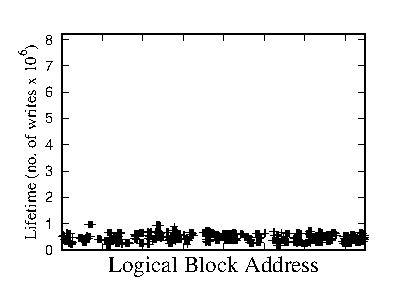
\includegraphics[width=0.4\textwidth]{figure/pcstream/type_4_new.eps}}  % data from 4/03040047
	\hspace{10pt}
\subfloat[RocksDB: L4 Compaction]{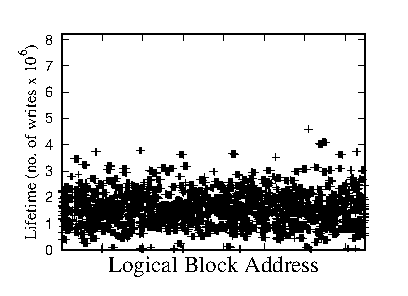
\includegraphics[width=0.4\textwidth]{figure/pcstream/type_6_new.eps}}
%\caption{The lifetime distribution of the compaction activity.} 
\caption{Lifetime distributions of the compaction activity at different levels.} %shane part
\label{fig:compaction}
\end{figure}




Unfortunately, in the current RocksDB implementation, the compaction step is supported 
by the same execution path ({\it i.e.}, the same PC) regardless of the level.
Therefore, the PC for the compaction activity cannot effectively separate data with 
short lifetimes from one with long lifetimes.
Fig.~\ref{fig:compaction}(a) and ~\ref{fig:compaction}(b) show
distinctly different lifetime distributions based on the level of compaction:
data written from the level 4 have a large lifetime variance while data written from
the level 2 have a small lifetime variance.

Similarly, in SQLite and GCC, program contexts with large lifetime variations
are also observed.
Fig.~\ref{fig:types_and_PCs}(e) shows large lifetime variances of data files in
SQLite.
Since client request patterns will decide how SQLite updates its tables, 
the lifetime of data from the updating activity of SQLite is distributed 
with a large variance.  Similarly, the lifetime of
data from the outputting temporary files of GCC can significantly fluctuate 
as well depending on when the next compile step starts.   
Fig.~\ref{fig:types_and_PCs}(g) shows long lifetimes of 
object files/executable files after 
a Linux build was completed
(with no more re-compiling jobs).
However, the lifetime of the same object files/executable files 
may become short when if we have to restart the same
compile step right after the previous one is finished
({\it e.g.}, because of code changes).

For these {\it outlier} PCs with large lifetime variations, 
it is a challenge to allocate streams in an efficient fashion unless 
there are more application-specific hints ({\it e.g.}, the compaction level in
RocksDB) are available.  
As an ad-hoc (but effective) solution, when a PC shows a large variance 
in its data lifetime, we allocate an additional stream, called an internal stream, 
to the PC so that
the data written from the PC can be better separated between the original 
stream and its internal stream.  
In order to support internal streams, the total number of streams may 
need to be doubled so
that each stream can be associated with its internal stream.

\subsection{Implementation of Internal Streams}
As described in Section~\ref{sec:limitedstreams}, it is difficult to increase the number of 
(normal) streams.  However, 
if we restrict that internal streams are used only for data movements
during GC,
they can be quite efficiently
implemented without the constraints on the backup power capacity and fast memory size.  
The key difference in the implementation overhead between normal streams and 
internal streams comes from a simple observation that data copied during 
GC do not need the same reliability and performance support as for host writes.  
Unlike buffered data from host write requests, valid pages in
the source block during garbage collection have no risk of losing their data 
from the sudden power-off conditions because the original valid pages are always available.    
Therefore, even if the
number of internal streams increases, unlike normal streams, 
no higher-capacity backup capacitor is necessary for managing buffered data for internal streams. 

The fast memory requirement is also not directly increased as the number 
of internal streams increases.   
Since internal streams are used only for GC and most GC can be handled as background tasks,
internal streams has a less stringent performance requirement.  
Therefore, data structures for supporting internal streams can be placed 
on DRAM without much performance issues.  
Furthermore, for a read request, there is no need to check if a read request 
can be served by buffered data as in normal streams because the source block always 
has the most up-to-date data.  
This, in turn, allows data structures for internal streams to be located in slow memory.
Once an SSD reaches the fully saturated condition where host writes and GC 
are concurrently performed, the performance of GC may degrade a little because of
the slow DRAM used for internal streams.   
However, in our evaluation, such cases were rarely observed under a 
reasonable overprovisioning storage capacity.


\section{Design and Implementation of \textsf{PCStream}}

\begin{figure}[t]
	\centering
	%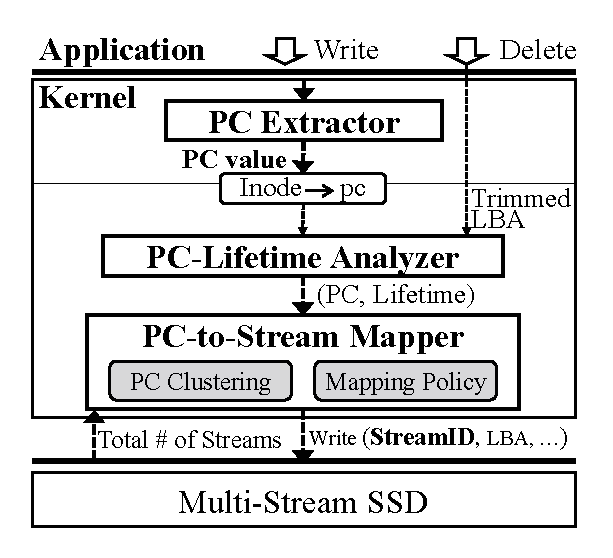
\includegraphics[width=0.6\linewidth]{figure/architecture4}
	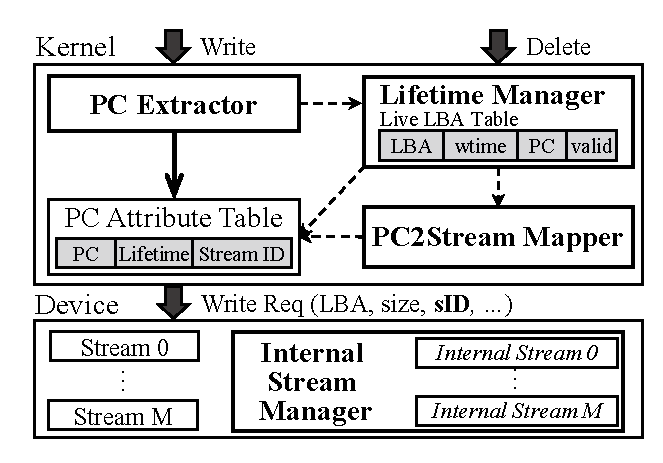
\includegraphics[width=0.8\linewidth]{figure/pcstream/overview_1}
	\caption{An overall architecture of \textsf{\small PCStream}.}
	\label{fig:architecture}
\end{figure}

% stream tbl (X)
% 4.2 -> 5
% short-lived app (X)
% training?

In this section, we explain the detailed implementation of \textsf{\small
PCStream}.  Fig.~\ref{fig:architecture} shows an overall architecture of
\textsf{\small PCStream}. The \textit{PC extractor} is implemented as part of a
kernel's system call handler as already described in
Section~\ref{sec:programcontext}, and is responsible for computing a PC
signature from applications.  The PC signature is used for deciding the
corresponding stream ID\footnote{ We call {\it i} the stream ID of $S_i$.} from
the PC attribute table.  \textsf{\small PCStream} maintains various per-PC
attributes in the PC attribute table including PC signatures, expected data
lifetimes, and stream IDs.  In order to keep the PC attribute table updated
over changing workloads, the computed PC signature with its LBA information is
also sent to the {\it lifetime manager}, which estimates expected lifetimes of
data belonging to given PCs.  Since commercial multi-streamed SSDs only expose
a limited number of streams to a host, the \textit{PC2Stream mapper} groups PCs
with similar lifetimes using a clustering policy, assigning PCs in the same
group to the same stream.  Whenever the lifetime manager or the PC2Stream
mapper are invoked, the PC attribute table is updated with new outputs from
these modules.  Finally, the \textit{internal stream manager}, 
which was implemented inside an SSD as a firmware, is responsible for
handling internal streams associated with external streams.

%the lifetime of data written by write-related system calls can be
%monitored at the program context level.  
%A PC signature value is stored in an
%inode data structure of a file system (modified for \textsf{\small PCStream})
%and is delivered to \textit{the lifetime analyzer module} which estimates
%expected lifetimes of data belonging to a given PC in the block device level.
%In order to efficiently detect the end of data lifetime in append-only
%workloads, the lifetime analyzer also intercepts TRIM~\cite{TRIM} requests from
%a file system.

%shane part Based on the lifetime information, \textit{the PC-to-stream mapper
%module} clusters PCs with similar lifetimes and maps them together to the same
%stream ID.  This mapping is required because the number of streams in an SSD
%is generally less than the number of PCs in host applications.

\subsection{PC Lifetime Management}
\label{sec:PC_lf_mngm}
The responsibility of the lifetime manager is for estimating the lifetime of
data associated with a PC. 
Except for outlier PCs, most data from the same PC tend to show similar 
data lifetimes with small variances.

\textbf{Lifetime estimation:}
Whenever a new write request {\it R} arrives, the lifetime manager stores the
write request time, the PC signature, $PC_i$, and the LBA list of {$R$} into
the live LBA table.  The live LBA table, indexed by an LBA, is used in
computing the lifetime of data stored at a given LBA which belongs to $PC_i$.
Upon receiving TRIM commands (that delete previously written LBAs) or overwrite
requests (that update previously written LBAs), the lifetime manager searches
the live LBA table for a PC signature $PC_{found}$ with the LBA list which
includes the deleted/updated LBAs.  The new lifetime $l_{new}$ of $PC_{found}$
is estimated using the lifetime of the matched LBA from the live LBA table. The
weighted average of the existing lifetime $l_{old}$ for $PC_{found}$ and
$l_{new}$ is used to update the $PC_{found}$ entry in the PC attribute table.
Note that the written time entry of the live LBA table is updated differently
depending on TRIM commands or overwrite requests.  The written time entry
becomes invalid for TRIM while it is updated by the current time for
an overwrite request.

Maintaining the live LBA table, which is indexed by an LBA unit, in DRAM could
be a serious burden owing to its huge size. In order to mitigate the DRAM
memory requirement, the lifetime manager slightly sacrifices the accuracy of
computing LBA lifetime by increasing the granularity of LBA lifetime prediction
to 1 MB, instead of 4 KB.  The live LBA table is indexed by 1 MB LBA, and each
table entry holds PC signatures and written times over a 1 MB LBA range.
Because of the coarse-grained indexing, each entry could have multiple
signatures and written times, and the same PC could span across multiple
entries.  If the same PC has different lifetimes, we take the arithmetic mean
as the PC lifetime.  To limit the table size, if the table reaches a threshold
size, the least recently referenced entry is evicted from the LBA table.
Currently, the threshold is set to 64 MB.

\textbf{PC attribute table:}
The PC attribute table keeps PC signatures and its expected lifetimes. To
quickly retrieve the expected lifetime of a requested PC signature, the PC
attribute table is managed through a hash data structure. Each hash entry
requires only 12 bytes: 64-bit for a PC signature and 32-bit for a predicted
lifetime.  The table size is thus small so that it can be entirely loaded
in DRAM.  From our evaluations, the DRAM size of the PC attribute table was
sufficient with several tens or hundreds of KB.

In addition to the main function of the PC attribute table that maintains the
data lifetime for a PC, the $memory-resident$ PC attribute table has another
interesting benefit for the efficient stream management.  Since a PC
signature of an I/O activity is virtually guaranteed to be {\it globally unique} across
{\it all} applications (the uniqueness property), and a PC signature does not change
over different executions of the same application (the consistency property), the PC
attribute table can capture a long-term history of programs' I/O behaviors.
Because of the uniqueness and consistency of a PC signature, \textsf{\small PCStream}
can exploit the I/O behavior of even short-lived processes ({\it e.g.}, \texttt{cpp}
and \texttt{cc1} for GCC)  that are launched and terminated frequently.  When
short-lived processes are frequently executed, the PC attribute table can hold
their PC attributes from their previous executions, thus enabling quick but
accurate stream allocation for short-lived processes.

The consistency property is rather straightforward because each PC signature is
determined by the sum of return addresses inside a process's virtual address
space.  Unless a program's binary is changed after recompilation, those return
addresses remain the same, regardless of program's execution.  The uniqueness property 
is also somewhat obvious from the observation that the probability that
distinct I/O activities that take different function-call paths have the same
PC signature is extremely low. This is even true for multiple programs. Even
though they are executed in the same virtual address space, it is very unlikely
that I/O activities of diverged programs taking different function-call paths
have the same PC.  Consequently, this immutable property of the PC signature
for a given I/O activity makes it possible for us to characterize the given I/O
activity in a long-term basis without a risk of PC collisions.

%The PC is determined by the sum of the return address, i.e., the path to reach
%the write system call.  In general, different I/O activities can not have the
%same return address because they are implemented in different functions.
%Since the probability that the sum of the different return addresses becomes
%the same is very low, the PC of an I/O activity in the same program is unique.
%For multiple programs, however, since each program uses a virtual address,
%several identical return addresses can occur.  However, the probability that
%two independent programs will have the same function call path over four or
%five is also very low, so we can usually say that a PC is unique.  Moreover,
%since the virtual address of the code is not changed after the compilation,
%the PC value will be the same when the program execution is terminated and
%restarted.  PCs of restarted program will be the same as the one of previous
%execution, and the life characteristics of the PC are also the same.  Because
%PCs are unique, if PC lifetime information is maintained, appropriate stream
%can be allocated even to the first request of a restarting program.

\subsection{Mapping PCs to SSD streams}

After estimating expected lifetimes of PC signatures, the PC2Stream mapper
attempts to group PCs with similar lifetimes into an SSD stream.  This grouping
process is necessary because while commercial SSDs only support a limited
number of streams ({\it e.g.,} 9), the number of unique PCs can be larger ({\it e.g.},
30).  For grouping PCs with similar lifetimes, the PC2Stream mapper module
uses the k-means algorithm~\cite{kmeans} which is widely used for similar
purposes.  In \textsf{\small PCStream}, we use the difference in the data
lifetime between two PCs as a clustering distance and  generates {\it m}
clusters of PCs for $m$ streams.  This algorithm is particularly well suited
for our purpose because it is lightweight in terms of the CPU cycle and
memory requirement.  To quickly assign a proper stream to incoming data, we add
an extra field to the PC attribute table which keeps a stream ID for each PC
signature.  More specifically, when a new write request comes, a designated SSD
stream ID is obtained by referring to the PC attribute table using request's PC
value as an index.  If there is no such a PC in the table, or a PC does not
have a designated stream ID, the request gets default stream ID, which is set
to 0.

For adapting to changing workloads, re-clustering operations should be
performed regularly. This re-clustering process is done in a straightforward
manner. The PC2Stream mapper scans up-to-date lifetimes for all PCs in the PC
attribute table. Note that PC's lifetimes are updated whenever the lifetime
manager gets new lifetimes while handling overwrites or TRIM requests, as
explained in Section~\ref{sec:PC_lf_mngm}.  With the scanned information, the PC2Stream mapper
recomputes stream IDs and updates stream fields of the PC attribute table.  In
order to minimize unnecessary overhead of frequent re-clustering operations,
re-clustering is triggered when 10\% of the PC lifetime entries in the PC
attribute table is changed.


\subsection{Internal Stream Management}
As explained in Section~\ref{sec:largevariance}, there are a few outlier PCs with large lifetime
variances. In order to treat these PCs in an efficient fashion, we devise a
two-phase method that decides SSD streams in two levels: the main stream in the
host level and its internal stream in the SSD level.  Conceptually, long-lived
data in the main stream are moved to its internal stream so that (future)
short-lived data will not be mixed with long-lived data in the main stream.
Although moving data to the internal stream may increase WAF, the overhead can
be hidden if we restrict data copies to the internal stream during GC only.
Since long-lived data ({\it i.e.}, valid pages) in a victim block are moved to a free
block during GC, blocks belong to an internal stream tend to contain long-lived
data.  For instance, \textsf{\small PCStream} assigns the compaction-activity
{\it $PC_1$} to a main stream {\it $S_1$} in the first phase.  To separate the
long-lived data of {\it $PC_1$} ({\it e.g.}, L4 data) from future short-lived data of
the same {\it $PC_1$} ({\it e.g.}, L1 data), valid pages of the {\it $S_1$} are
assigned to its internal stream for the second phase during GC.

We have implemented the internal stream manager with the two-phase method in
Samsung's PM963 SSD~\cite{PM963}. To make it support the two-phase method, we
have modified its internal FTL so that it manages internal streams while
performing GC internally.  Since the internal stream manager assigns blocks for
an internal stream and reclaims them inside the SSD, no host interface changed
is required.

%{\color{blue} 추가로, SSD가 지원하는 stream의 개수가 변경되는 상황에서도
%reclustering을 통해
%대응이 가능하다.
%reclustering의 주기는 workload의 변화 패턴에 따라 결정될 수 있다.
%새로운 PC가 계속적으로 생성되거나 한 PC의 수명 패턴이 자주 변화할 경우 reclustering의 주기를 
%좀 더 짧게 설정하여 workload 변화를 반영한다.
%}
%Since the
%number of PCs created by applications is not limited, the clustering algorithm
%must be efficient enough to quickly handle many PCs. 

\subsection{PC Extraction for Indirect Writes}
One limitation of using PCs to extract I/O characteristics is that it only
works with C/C++ programs that \textit{directly} call write-related system
calls.  Many programs, however, often invoke write system calls
\textit{indirectly} through intermediate layers, which makes it difficult to
track program contexts.

The most representative example may be Java programs, such as Cassandra, that
run inside a Java Virtual Machine (JVM). Java programs invoke write system
calls via the Java Native Interface (JNI)~\cite{JNI} that enables Java programs
to call a native I/O library written in C/C++.  For Java programs, therefore, the
PC extractor shown in Fig.~\ref{fig:architecture} fails to capture Java-level
I/O activities as it is unable to inspect the JVM stack from the native write
system call which is indirectly called through the JNI.  Another example is a
program that maintains a write buffer that is dedicated to dealing with all the
writes from an application. For example, in MySQL~\cite{MySQL} and
PostgreSQL~\cite{PostgreSQL}, every write is first sent to a write buffer.
Separate flush threads later materialize buffered data to persistent storage.
In that case, the PC extractor only captures PCs of flush threads, not PCs of
I/O activities that originally generate I/Os, because the I/O activities were
executed in different threads using different execution stacks.

\begin{figure}[t]
\centering
	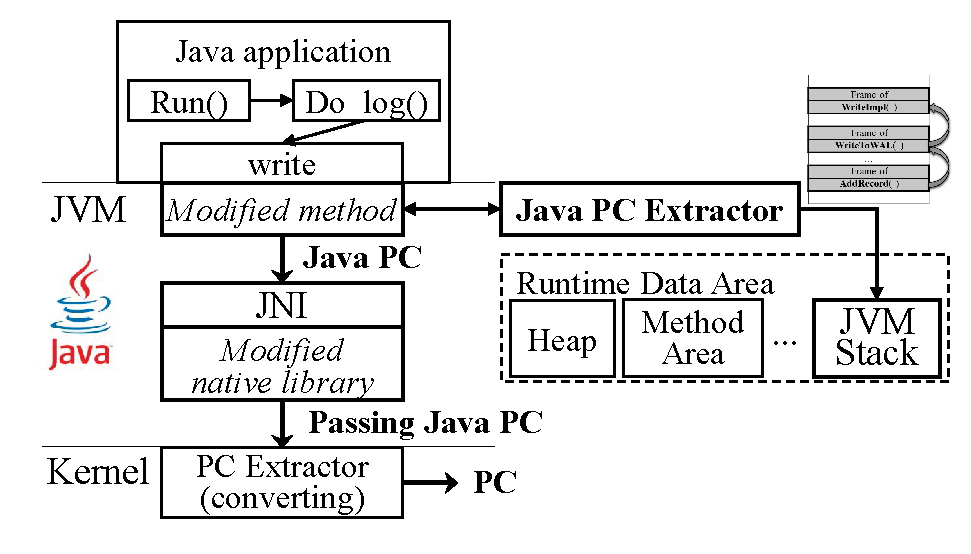
\includegraphics[width=0.7\linewidth]{figure/pcstream/jvmpc}
	\caption{Extracting PCs for JVM.}
\label{fig:java}
\end{figure}

The problem of indirect writes can be addressed by collecting PC signatures
{\it at the front-end interface} of an intermediate layer that accepts write
requests from other parts of the program. In case of Java programs, a native
I/O library can be modified to capture write requests and computes their PC
signatures. Once a native library is modified, \textsf{\small PCStream} can
automatically gather PC signatures without modifying application programs.
Fig.~\ref{fig:java} illustrates how \textsf{PCStream} collects PC signatures
from Java programs.  We have modified the OpenJDK~\cite{OpenJDK} source to
extract PC signatures for most of write methods in write related classes, such
as \texttt{OutputStream}.  The stack area in the \texttt{Runtime Data Areas} of
JVM is used to calculate PC signatures.  The calculated PC is then passed to
the write system call of the kernel via the modified native I/O libraries.

Unlike Java, there is no a straightforward way to collect PCs from applications
with write buffers. This is because the implementation of write buffering is
different depending on applications. Additional efforts to manually modify code
are unavoidable. However, the scope of this manual modification is limited only
to the write buffering code, and application logics themselves don't need to be
edited or annotated.


\section{Experimental Results}
\subsection{Experimental Settings}
In order to evaluate \textsf{\small PCStream}, we have implemented it in the
Linux kernel (version 4.5) on a PC host with Intel Core i7-2600 8-core
processor and 16~GB DRAM.  As a multi-streamed SSD, we used Samsung's PM963
480~GB SSDs.  The PM963 SSD supports up to 9 streams; 8 user-configurable
streams and 1 default stream.  When no stream is specified with a write
request, the default stream is used.  To support internal streams, we have
modified the existing PM963 FTL firmware.  For a detailed performance analysis,
we built a modified {\tt nvme-cli}~\cite{nvmecli} tool that can retrieve the internal
profiling data from \textsf{\small PCStream}-enabled SSDs.  
Using the modified {\tt nvme-cli} tool, we can monitor 
WAF values and per-block data lifetimes from the extended PM963 SSD during run time.

We compared \textsf{\small PCStream} with three existing schemes:
\textsf{\small Baseline}, \textsf{\small ManualStream}~\cite{MultiStream}, and
\textsf{\small AutoStream}~\cite{AutoStream}.  \textsf{\small Baseline}
indicates a legacy SSD that does not support multiple streams. \textsf{\small
ManualStream} represents a multi-streamed SSD with manual stream allocation.
\textsf{\small AutoStream} represents the LBA-baed stream management technique
proposed in ~\cite{AutoStream}. 


We have carried out experiments with various benchmark programs
which represent distinct write characteristics.
RocksDB~\cite{RocksDB} and Cassandra~\cite{Cassandra} have
append-only write patterns. SQLite~\cite{SQLite} has in-place update write patterns
and GCC~\cite{GCC} has write-once patterns.  
For more realistic evaluations, we also used mixed workloads running two 
different benchmark programs simultaneously.

In both RocksDB and Cassandra experiments, Yahoo! Cloud Serving Benchmark
(YCSB)~\cite{YCSB} with 12-million keys was used to generate update-heavy
workloads (workload type A) which consists of 50/50 reads and writes.  Since
both RocksDB and Cassandra are based on the append-only LSM-tree
algorithm~\cite{LSM}, they have three dominant I/O activities (such as logging,
flushing, and compaction).  Cassandra is written in Java, so its PC is
extracted by the modified procedure described in Section~\ref{sec:internal}.  In SQLite evaluations,
TPC-C~\cite{TPCC} was used with 20 warehouses.  SQLite has two dominant I/O
activities such as logging and updating tables.  In GCC experiments, a Linux
kernel was built 30 times.  For each build, 1/3 of source files, which were
selected randomly, were modified and recompiled.  Since GCC creates many
temporary files ({\it e.g.}, \texttt{.s}, \texttt{.d}, and \texttt{.rc}) as
well as long-lived files ({\it e.g.}, \texttt{.o}) from different compiler
tools, there are more than 20 dominant PCs.  To generate mixed workloads, we run
RocksDB and GCC scenarios together (denoted by Mixed 1), and run SQLite and GCC
scenarios at the same time (denoted by Mixed 2).  In order to emulate an aged
SSD in our experiments, 90\% of the total SSD capacity was initially filled up
with user files before benchmarks run.

\subsection{Performance Evaluation}

\begin{figure}[t]
	\centering
	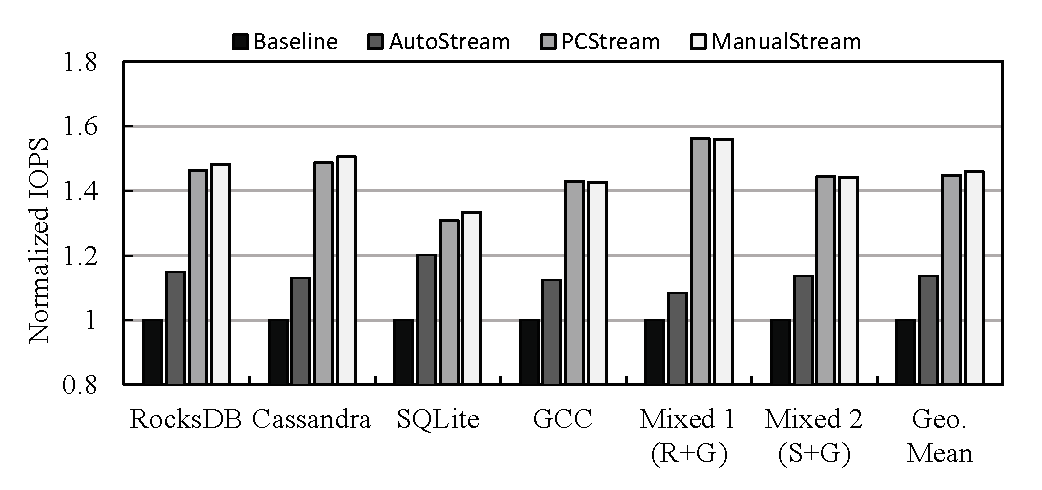
\includegraphics[width=1\linewidth]{figure/pcstream/iops}
	\caption{A comparison of normalized IOPS.}
	\label{fig:iops}
\end{figure}

We compared IOPS values of three existing techniques with \textsf{\small
PCStream}.  Fig.~\ref{fig:iops} shows normalized IOPS for six benchmarks with
four different techniques. For all the measured IOPS values\footnote{ For
RocksDB, Cassandra, and SQLite, the YCSB benchmark and TPC-C benchmark compute
IOPS values as a part of the benchmark report.  For GCC,
where an IOPS value is not measured during run time, 
we computed the IOPS value as a ratio between the total number of write requests
(measured at the block device layer) and the total elapsed time of running GCC.},
\textsf{\small PCStream} improved the average IOPS by 45\% and 28\% over 
\textsf{\small Baseline} and \textsf{\small AutoStream}, respectively.
\textsf{\small PCStream} outperformed \textsf{\small AutoStream}
by up to 56\% for complex workloads ({\it i.e.}, GCC, Mixed1 and Mixed 2) where
the number of extracted PCs far exceeds the number of supported streams
in PM963. The high efficiency of \textsf{\small PCStream} under complex
workloads comes from two novel features of \textsf{\small PCStream}: (1) LBA-oblivious 
PC-centric data separation and (2) a large number of streams supported 
using internal streams. \textsf{\small AutoStream}, on the other hands,
works poorly except for SQLite where the LBA-based separation
can be effective.
Even in SQLite, \textsf{\small PCStream} outperformed \textsf{\small AutoStream}
by 10\%.

\subsection{WAF Comparison}

Fig.~\ref{fig:waf} shows WAF values of four techniques for six benchmarks.
Overall, \textsf{\small PCStream} was as efficient as \textsf{\small
ManualStream}; Across all the benchmarks, \textsf{\small PCStream} showed 
similar WAF values as \textsf{\small ManualStream}. \textsf{\small PCStream}
reduced the average WAF by 63\% and 49\% over \textsf{\small Baseline} and
\textsf{\small AutoStream}, respectively.  

As expected, \textsf{\small Baseline} showed the worst performance among all
the techniques. Owing to the intrinsic limitation of LBA-based data
separation, \textsf{\small AutoStream} performs poorly except for
SQLite.  Since \textsf{\small PCStream} (and \textsf{\small ManualStream}) did
not depend upon LBAs for stream separations, they performed well consistently,
regardless of write access patterns. As a result, \textsf{\small PCStream}
reduced WAF by up to 69\% over \textsf{\small AutoStream}.

%Only SQLite had in-place update patterns for log files, 
%but the larger amount of data were written to database files 
%whose lifetimes are determined by the client
%which makes hard to predict their lifetime by the address.  In PCStream,
%however, long-lived data in database files are moved to internal streams during
%GC so that we can further reduce WAF.

One interesting observations in Fig.~\ref{fig:waf} is that \textsf{\small
PCStream} achieved a lower WAF value than even \textsf{\small ManualStream} for
GCC, Mixed 1, and Mixed 2 where more than the maximum number of streams in
PM963 are needed.  In \textsf{ManualStream}, DB applications and GCC were
manually annotated at offline, so that write system calls were statically bound
to specific streams during compile time.  When multiple programs run together
as in three complex workloads ({\it i.e.}, GCC, Mixed 1 and Mixed 2), static stream
allocations are difficult to work efficiently because they cannot adjust to
dynamically changing execution environments.  However, unlike \textsf{\small
ManualStream}, \textsf{\small PCStream} continuously adapts its stream
allocations during run time, thus quickly responding to varying execution
environments.

\begin{figure}[t]
	\centering
	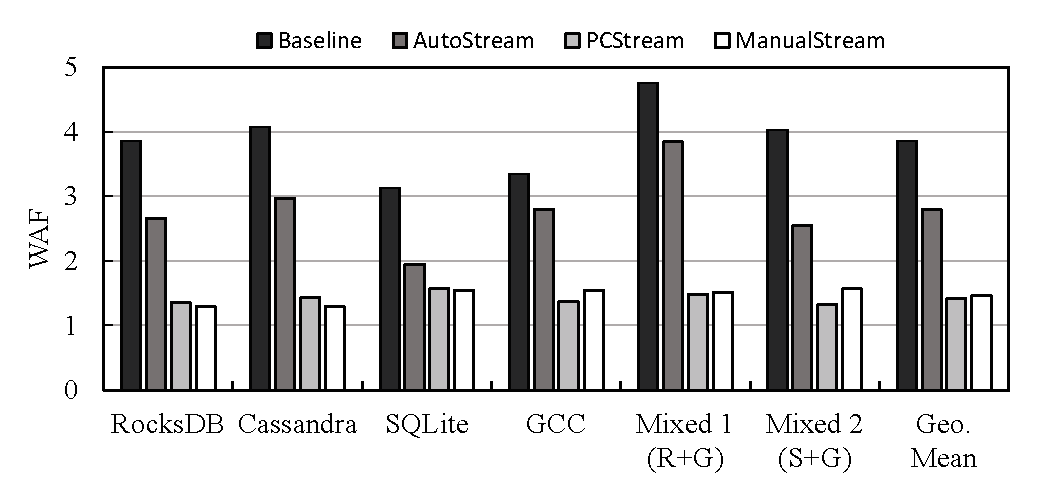
\includegraphics[width=1.\linewidth]{figure/pcstream/waf}
	\caption{A comparison of WAF under different schemes.}
	\label{fig:waf}
\end{figure}


%since the Manual scheme has static stream allocation.
%In Manual, once data types is mapped to the stream, the mapping is not changed 
%during runtime.
%For complex workloads which have large number of PCs such as mixed cases,
%it is difficult to expect data lifetimes in detail based on the data types.
%If the lifetime pattern is changed during runtime or the programmer choose
%second best stream mapping,
%Manual scheme lose the potential benefit in reducing WAf.
%However, the reclustering enables PCStream to adapt changing workload or find
%better stream mapping.
%The detailed analysis will be shown in the following subsections.
\subsection{Per-stream Lifetime Distribution Analysis}

To better understand the benefit of \textsf{\small PCStream} on the WAF
reduction, we measured per-stream lifetime distributions for the Mixed 1
scenario.  Fig.~\ref{fig:distribution} shows a box plot of data lifetimes from
the 25th to the 75th percentile.  As shown in Fig.~\ref{fig:distribution},
streams in both \textsf{\small PCStream} and \textsf{\small ManualStream} are
roughly categorized as two groups, $G1$ = $\{S_1$, $S_2$, $S_3$, $S_4$, $S_5\}$
and $G2$ = $\{S_6$, $S_7$, $S_8\}$, where $G1$ includes streams with short
lifetimes and small variances ({\it i.e.}, $S_1$, $S_2$, $S_3$, $S_4$, and $S_5$) and
$G2$ includes streams with large lifetimes and large variances ({\it i.e.}, $S_6$,
$S_7$, and $S_8$). The $S_0$ does not belong to any groups as it is assigned to
requests whose lifetimes are unknown.  Even though the variance in the $S_0$ is
wider than that in \textsf{\small ManualStream}, \textsf{\small PCStream}
showed similar per-stream distributions as \textsf{\small ManualStream}.  In
particular, for the streams in $G2$, \textsf{\small PCStream} exhibited smaller
variance than \textsf{\small ManualStream}, which means that \textsf{\small
PCStream} separates cold data from hot data more efficiently.  Since
\textsf{\small PCStream} moves long-lived data of a stream to its internal
stream, the variance of streams with large lifetimes tend to be smaller over
\textsf{\small ManualStream}.

\begin{figure}[t]
	\centering
	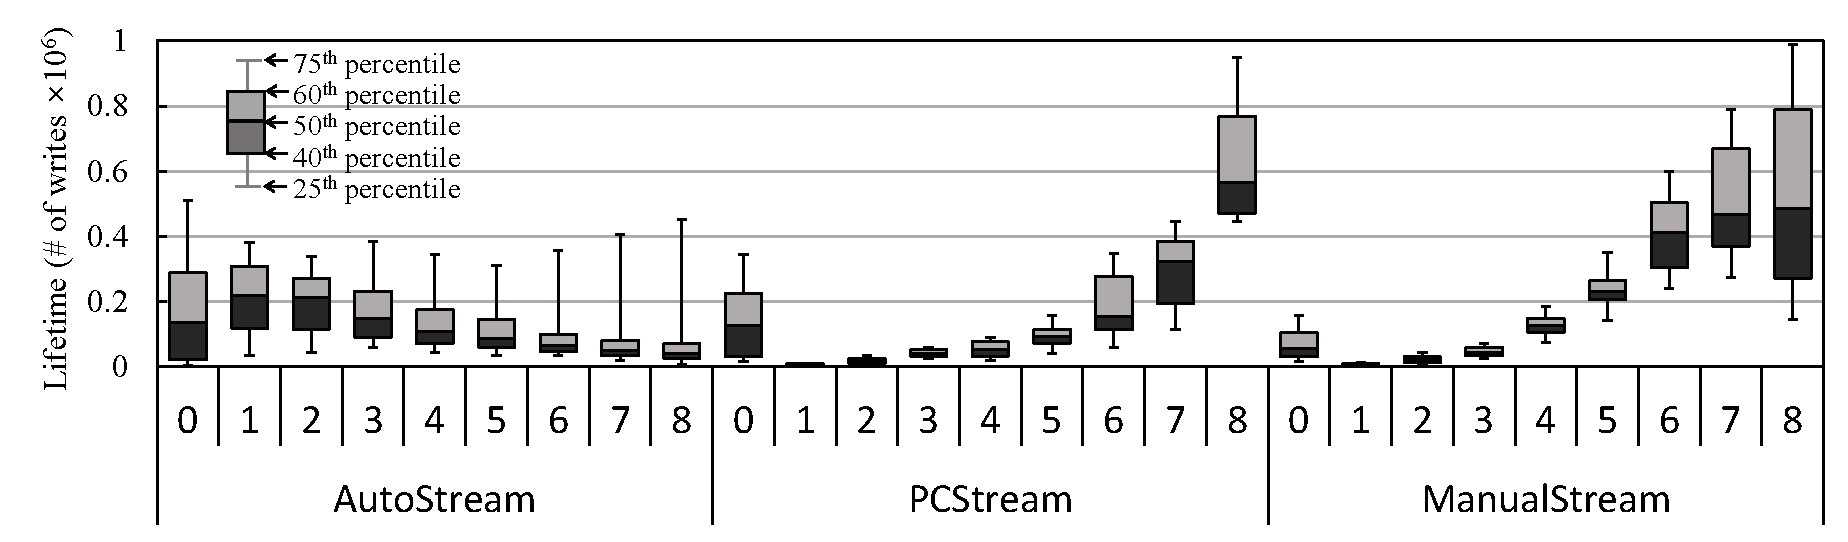
\includegraphics[width=1\linewidth]{figure/pcstream/distribution}
	\caption{A Comparison of per-stream lifetime distributions.}
	\label{fig:distribution}
\end{figure}


\textsf{\small AutoStream} was not able to achieve small per-stream variances
as shown in Fig.~\ref{fig:distribution} over \textsf{\small PCStream} and
\textsf{\small ManualStream}.  As shown in Fig.~\ref{fig:distribution}, all the
streams have large variances in \textsf{\small AutoStream} because hot data are
often mixed with cold data in the same stream.  Since the LBA-based data
separation technique of \textsf{\small AutoStream} does not work well with both
RocksDB and GCC, all the streams include hot data as well as cold data, thus
resulting in large lifetime variances. 

\subsection{Impact of Internal Streams}
\begin{figure}[t]
	\centering
	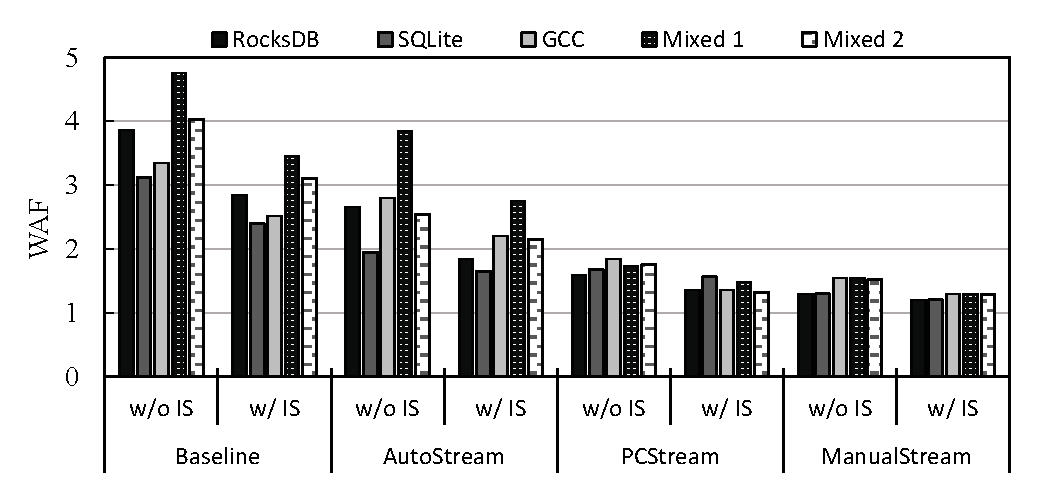
\includegraphics[width=1.\linewidth]{figure/pcstream/internal}
	\caption{The effect of internal streams on WAF.}
	\label{fig:internal}
\end{figure}

In order to understand the impact of internal streams on different stream
management techniques, we compared the two versions of each technique, one with
internal streams and the other without internal streams.  Since internal
streams are used only for GC, they can be combined with any
existing stream management techniques.  Fig.~\ref{fig:internal} shows WAF values
for five benchmarks with four techniques.  Overall, internal streams worked
efficiently across the four techniques evaluated.   When combined with
internal streams, \textsf{\small Baseline}, \textsf{\small AutoStream},
\textsf{\small PCStream} and \textsf{\small ManualStream} reduced the average
WAF by 25\%, 22\%, 17\%, and 12\%, respectively.  Since the quality of initial
stream allocations in \textsf{\small Baseline} and \textsf{\small AutoStream}
was relatively poor, their WAF improvement ratios with internal streams were
higher over \textsf{\small PCStream} and \textsf{\small ManualStream}.
Although internal streams were effective in separating short-lived data from
long-lived data in both \textsf{\small Baseline} and \textsf{\small
AutoStream}, the improvement from internal streams in these techniques are not
sufficient to outperform \textsf{\small PCStream} and \textsf{\small
ManualStream}.  Poor initial stream allocations, which keep putting both hot
and cold data to the same stream, unfortunately, offset a large portion of
benefits from internal streams.



\subsection{Impact of the PC Attribute Table}
As explained in Section~\ref{sec:PC_lf_mngm}, the PC attribute table is useful to maintain a
long-term history of applications' I/O behavior by exploiting the uniqueness of
a PC signature across different applications.   To evaluate the effect of the
PC attribute table on the efficiency of \textsf{\small PCStream}, we modified
the implementation of the PC attribute table so that the PC attribute table can
be selectively disabled on demands when a process terminates its execution.
For example, in the kernel compilation scenario with GCC, the PC attribute
table becomes empty after each kernel build is completed.  That is, the next
kernel build will start with no existing PC to stream mappings.


\begin{figure}[t]
	\centering
	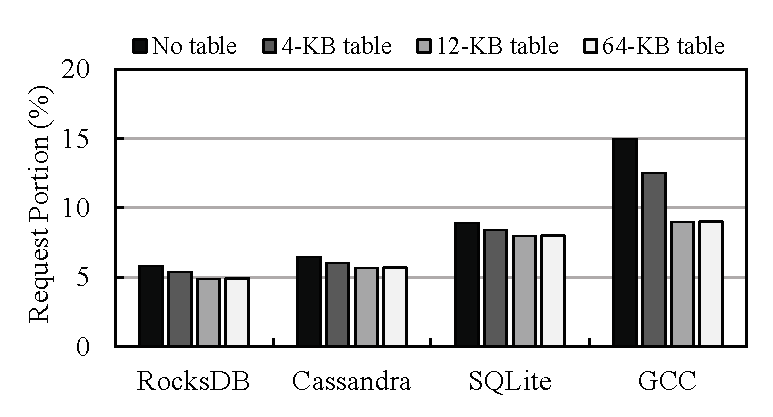
\includegraphics[width=1\linewidth]{figure/pcstream/pctable}
	%\caption{The effect of the PC attribute table on the default stream allocation.}
	\caption{The effect of the PC attribute table.}
	\label{fig:pctable}
\end{figure}

Fig.~\ref{fig:pctable} show how many requests are assigned to the default
$S_{0}$ stream over varying sizes of the PC attribute table.  Since $S_{0}$ is
used when no stream is assigned for an incoming write request, the higher the
ratio of requests assigned to $S_{0}$, the less effective the PC attribute
table.   As shown in Fig.~\ref{fig:pctable}, in RocksDB, Cassandra, and SQLite,
the PC attribute table did not affect much the ratio of writes on $S_{0}$.
This is because these programs run continuously for a long time while
performing the same dominant activities repeatedly.  Therefore, although the PC
attribute table is not maintained, they can quickly reconstruct it.  On the
other hand, the PC attribute table was effective for GCC, which frequently
creates and terminates multiple processes ({\it e.g.}, {\tt cc1}).  When no PC
attribute table was used, about 16\% of write requests were assigned to
$S_{0}$.  With the 4-KB PC attribute table, this ratio was reduced to 12\%.
With the 12-KB PC attribute table, only 9\% of write requests were assigned to
$S_{0}$.  This reduction in the $S_{0}$ allocation ratio reduced the WAF value
from 1.96 to 1.54.


